\documentclass[a4j,dvipdfmx]{jarticle}
%----------------------------------------------------------------------
\usepackage{graphicx}
\usepackage{amsmath}
\usepackage{amssymb}
\usepackage{bm}
\usepackage{fancybox}
\usepackage{fancyhdr}
\usepackage{lastpage}
\usepackage{color}
\usepackage{multicol}
\usepackage{listings,jlisting}
%----------------------------------------------------------------------
\setlength{\topmargin}{-0.5in}
%\addtolength{\headheight}{1cm}
%%\setlength{\headsep}{0mm}
%\setlength{\oddsidemargin}{-0.5in}
%%\setlength{\evensidemargin}{-0.5in}
%\addtolength{\textwidth}{1.5in}
\addtolength{\textheight}{1in}
%----------------------------------------------------------------------
%\setlength{\columnsep}{2zw}
%\setlength{\columnseprule}{0.4pt}
%----------------------------------------------------------------------
\pagestyle{fancy}
\lhead{2016/04/12}
\rhead{(\thepage / \pageref{LastPage})}
\cfoot{}
\chead{\textgt{システムプログラミング2 課題2解答}}
%----------------------------------------------------------------------
\begin{document}
\def\lstlistingname{リスト}
\lstset{language=C,
%  numbers=left,
  basicstyle={\small\ttfamily},
%  basicstyle={\ttfamily},
  columns=[l]{fullflexible},
  keepspaces=true,
%  showspaces=true,
  frame=shadowbox
}

\begin{enumerate}
\item ソースコードと実行例

\lstinputlisting[caption=低水準I/O版のmycp(mycp2.c)]{mycp2.c}

\begin{lstlisting}[caption=実行例(動作テスト!!)]
$ mycp2                                     <-- コマンド行引数がない場合
Usage: mycp2 <srcfile> <dstfile>
$ mycp2 a.txt                               <-- コマンド行引数が一つしかない場合
Usage: mycp2 <srcfile> <dstfile>
$ mycp2 z.txt a.txt                         <-- コピー元が存在しない場合
z.txt: No such file or directory
$ mycp2 a.txt /a.txt                        <-- コピー先が書き込み禁止の場合
/a.txt: Permission denied
$ echo aaa bbb > a.txt                     <-- a.txt を作って
$ mycp a.txt b.txt                         <-- b.txt にコピーしてみる
$ cat b.txt                                <-- b.txt の内容を確認
aaa bbb
$ echo ccc ddd > c.txt                     <-- c.txt を作って
$ mycp c.txt b.txt                         <-- b.txt に上書きしてみる
$ cat b.txt                                <-- b.txt の内容を確認
ccc ddd
\end{lstlisting}

\newpage

\item 性能測定の手順を確認する。

「1MB(メガバイト($2^{20}$バイト))のファイルをコピーする時間」を測定したい。
以下のように{\tt dd}コマンドでファイルを作成して{\tt time}コマンドで
時間を測定しようと思う。
うまくできるか確認する。

\begin{lstlisting}[caption=性能測定手順]
$ dd if=/dev/random of=aaa bs=1024 count=1024
1024+0 records in
1024+0 records out
1048576 bytes transferred in 0.076589 secs (13690929 bytes/sec)
$ ls -l aaa
-rw-r--r--  1 sigemura  staff  1048576 Apr 23 11:32 aaa
$ time mycp2 aaa bbb
real	0m0.012s
user	0m0.001s
sys	0m0.008s
[sigemura@02_低水準IO]$ ls -l aaa bbb
-rw-r--r--  1 sigemura  staff  1048576 Apr 23 11:32 aaa
-rw-r--r--  1 sigemura  staff  1048576 Apr 23 11:33 bbb
\end{lstlisting}

\item 測定の結果

前の方法で 1MB のファイルをコピーする時間を測定してみる。
\verb/mycp/(高水準)、\verb/mycp2_1024/(低水準でBSIZ=1024)、
\verb/mycp2_1/(低水準でBSIZ=1)について何度か測定して平均を求めた。

\begin{multicols}{2}
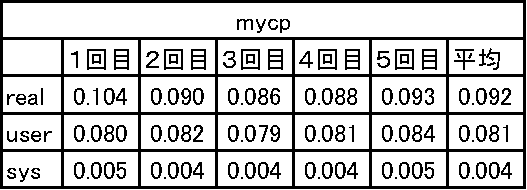
\includegraphics[scale=.7]{mycp_1M-crop.pdf}

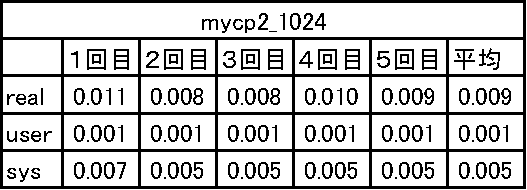
\includegraphics[scale=.7]{mycp2_1024_1M-crop.pdf}

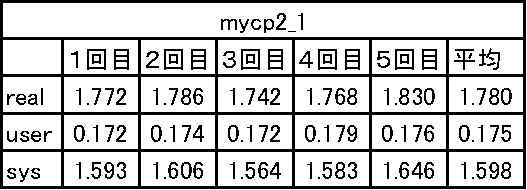
\includegraphics[scale=.7]{mycp2_1_1M-crop.pdf}

低水準でBSIZ=1が遅いことが分かる。
しかし、実行時間が短すぎて誤差の割合が高そうだ。

\end{multicols}

\item 再測定の結果

10MB のファイルをコピーする時間を測定した。

\begin{multicols}{2}
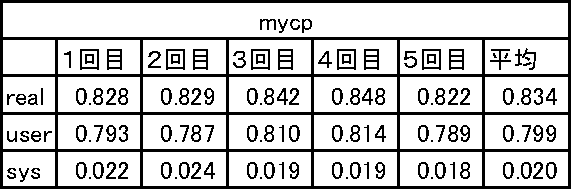
\includegraphics[scale=.7]{mycp_10M-crop.pdf}

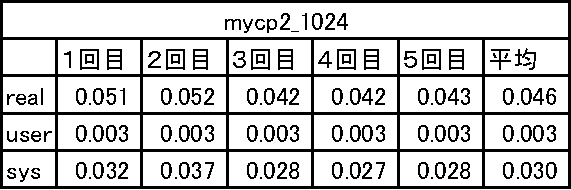
\includegraphics[scale=.7]{mycp2_1024_10M-crop.pdf}

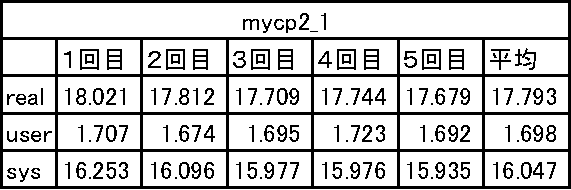
\includegraphics[scale=.7]{mycp2_1_10M-crop.pdf}

ファイルサイズを10倍にしても傾向は同じようだ。

1番:低水準でBSIZ=1024

2番:高水準

3番:低水準でBSIZ=1

\end{multicols}

\end{enumerate}
\end{document}

